\documentclass[12pt,a4paper]{article}
\usepackage{cmap}
\usepackage{amsmath}
\usepackage{mathtext}
\usepackage{titlesec}

\usepackage[utf8]{inputenc}
\usepackage[T2A]{fontenc}
\usepackage{wrapfig}
\usepackage[english, russian]{babel}
\usepackage[left=2cm,right=2cm,top=2cm,bottom=2cm]{geometry}
\usepackage{indentfirst}

\DeclareSymbolFont{T2Aletters}{T2A}{cmr}{m}{it}

%%% Работа с картинками
\usepackage{graphicx}  % Для вставки рисунков
\graphicspath{{imgs/}}  % папки с картинками

\usepackage{caption}
\captionsetup{labelsep=period, labelfont=bf}

\titleformat{\section}[block]
{\normalfont}{\thesection.}{0 cm}{}
\titleformat{\subsection}[block]
{\bfseries}{\thesubsection.}{0 cm}{}

\titlespacing{\section}{17pt}{14pt}{10pt}
\titlespacing{\subsection}{17pt}{14pt}{4pt}

\def \TITLE {Отчет о выполнении лабораторной работы №1.1.4}
\def \SUBTITLE {Измерение интенсивности радиационного фона}
\def \AUTHOR {Выполнил студент группы Б03-405\\ Тимохин Даниил}
\def \DATE {11 сентября 2024 г.}

\begin{document}

\begin{titlepage}
	\centering
	\vspace{5cm}
	{\scshape\large Московский физико-технический институт \\
	(НАЦИОНАЛЬНЫЙ ИССЛЕДОВАТЕЛЬСКИЙ УНИВЕРСИТЕТ)}
	
	\vspace{4cm}
	{\LARGE \TITLE}
	
	\vspace{1cm}
	{\Huge\bf \SUBTITLE }
	
	\vspace{1cm}
	\vfill
	
\begin{flushright}
	{\LARGE \AUTHOR}
\end{flushright}
	

	\vfill

	\DATE
\end{titlepage}

\newpage

\fontsize{12}{14}\selectfont

\section{ Аннотация}
В работе измеряется интенсивность радиационного фона у поверхности земли. Измерения производятся с помщью счетчика Гейгера-Мюллера (СТС-6). Детально исследуется статистическаие закономерности при измерении случайных величин. Отрабатываются навыки обработки эксперементальных данных.

\section{ Теоритические сведенья}

\subsection{ Космические лучи}
Основную часть радиоционного излучения составлет поток космических частиц, который изменяется со временем случайным образом.

Первичные космические лчуи - это поток стабильных частиц, имеющих большую кинетическую энергию, которая состовляет от $10^9$ эВ до $10^{21}$ эВ. В основном его составляют протоны(92\%) и $\alpha$-частицы(6,6\%), а также другие частицы. Число $\gamma$-квантов с энергиями больше $10^8$ эВ составляет всего 0,01\%.
Установлено, что поток частиц одинаков по всем направлениям(изотропен).

При этом много частиц, попадая в атмосферу поглащаются ей, ионизируя её. При этом образуется вторичные космические лучи. Мягкая их компонента  почти не доходит до поверхности, но образуется там благодаря жёсткомой компоненте. Поэтому космические лучи у поверхности моря примерно в 100 раз менее плотны, чем в верхней границе атмосферы. При этом в среднем плотность потока космических лучей по исследовниям за последние 35 тысяч лет практически не изменилась. 

Измеряемая плотность потока сильно зависит от направления. Изменение приближенно пропорционально квадрату косинуса угла отклонения от вертикали, что связано с увеличением пути, проходимого лучами в атмосфере Земли. Но так как датчик, используемый в работе всенаправленный, то особого значения этот фактор на эксперимент не оказывает.

\subsection{ Устройство счетчика Гейгера-Мюллера}
\begin{wrapfigure}{r}{0.3\textwidth}
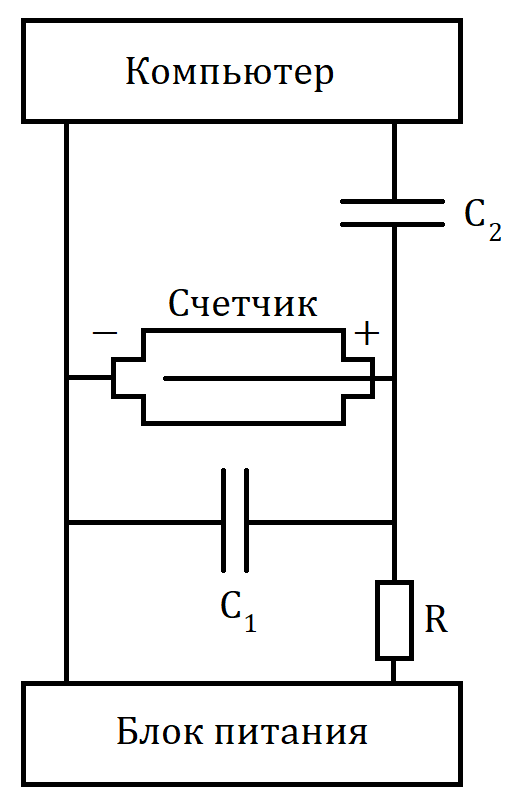
\includegraphics[width=0.3\textwidth]{imgs/scheme.png}
\caption{Схема подключения счетсика}
\label{fig:scheme}
\end{wrapfigure}
Для измерения интенсивности  космических лучей используется счётчик Гейгера-Мюллера. Его принцип работы основан на ионизации газа пролетающими через него частицами. Существует несколько типов таких счетчиков. Исспользуемый в данной работе (СТС-6) представляет собой тонкий металлический цилиндр, который является катодом, внутри которого протянута металлическая нить, являющаяся анодом. На электроды подаётся примерно 400В. Частицы космических лучей ионизируют газ. Высвободившиеся электроны ускоряются в электрическом поле и начинают ионизировать другие атомы газа. В результате образуется лавина  электронов, и через счетчик резко увеличивается ток.

Постоянное напряжение на счетчик подаётся через сопротивление $R$. СТС-6 и $C_1$ заряжены до напряжения 400В, так как сопротивление резистора много меньше сопротивления СТС-6 и конденсатора $C_1$. Конденсатор $C_2$ нужен, чтобы не пропускать постоянный ток на интерфейсные схемы компьютера.

При возникновении тока заряд на СТС-6 и $C_1$ обеспечивает развитие лавины электронной лавины на короткое время. В процессе разряда энергия поступает с $C_1$. Когда Когда разряд в счетчике прекращается, система начинает востанавливаться. Этот процесс занимает порядка нескольких $RC_1$. При этом через конденсатор $C_2$ передаст короткий сигнал на схему компьютера.

Конденсатор $C_1$ нужно выбрать так, чтобы запасённой энергии хватило на создание лавины, но при этом мёртвое время ($\tau \sim RC_1$) должно быть не слишком большим. Данным условиям соответствует ёмкость самого датчика, поэтому дополнительный конденсатор $C_1$ не потребуется. Сопротивление резистора R должно быть достаточным для быстрой зарядки конденсатора, но и не слишком большим,чтобы лавина электронов могла потухнуть. Обычно $R\sim1$ МОм.

Оценки показывают, что погрешность измерерний с помощью датчика Гейгера-Мюллера намного меньше, чем флуктуации самого потока частиц, а значит его можно считать в данной работе идеальным прибором.

\subsection{Определение погрешностей измерения плотности потока}
Так как прохождение частицей датчика является равновероятным независимым дискретным событием, то процесс можно считать пуассоновским, а результаты подчиняются распределению Пуассона. При этом для больших отсчётов(длительность по времени) распределение стремиться к нормальному.

При этом по теории вероятности для пуассоновского процесса вероятность $w_k$ получить $k$ зарегестрированных частиц в отсчёте при среднем количестве частиц $\lambda$
\begin{equation}
    w_k=\frac{\lambda^k}{k!}e^{-\lambda}.
\end{equation}
Из теории вероятности доказывается, что в таком процессе стандартную ошибку можно определить по формуле. $\sigma_k=\sqrt{\lambda}$.

Но будем оценивать по стандартной формуле и сравнивать с оценкой для пуассоновского процесса
\begin{equation}
\sigma _k = \sqrt{\frac{1}{N} \sum \left( k_i - \lambda \right)^2},
\end{equation}где $N$ - количество отсчётов.
При этом $\sigma_{\lambda}=\frac{\sigma _k}{\sqrt{N}}\approx\frac{\sqrt{\lambda}}{\sqrt{N}}$.

И относительая ошибка измерения $\varepsilon_{\lambda}=\frac{\sigma_{\lambda}}{\lambda} \approx \frac{1}{\sqrt{\lambda N}}$, а относительная ошибка оценки стандартной ошибки $\varepsilon_{\sigma}=\frac{\lvert \sigma _{\lambda}-\sqrt{\lambda} \rvert}{\sigma _{\lambda}}$

\section{Оборудование}

{\bfseries Модуль со счетчиком Гейгера-Мюллера СТС-6}

{\bfseries Программа для проведения эксперимента}

{\bfseries Дополнительный источник частиц} (Судя по показаниям датчика во время опыта он излучал $\alpha$ и слабое $\beta$ излучение)

\section{ Результаты измерений и обработка данных}
На компьютере была запущена рпограмма для расчета на 4000 с для измерений. Первый файл с именем $"exp1.txt"$ был создан с использованием источника в определенный момент времени примерно на 15 с. После был записан эксперимент без источника в $"exp2.txt"$. Сначала обработаем второй файл.

Введем обозначения:

$\tau$ -- длительность отсчёта, 

$N$ -- количество отсчётов,

$n$ -- количество частиц в отсчёте, 

$k_n$ -- Количество отсчётов равных $n$,

$\overline{n}$  -- среднее количество частиц в отсчётах, 

$\sigma_{n}$ -- ошибка отдельного отсчёта, 

$\sigma_{\overline{n}}$ -- ошибка среднего отсчёта, 

$\varepsilon_{\overline{n}}$ -- относительная ошибка среднего отсчёта, 

$w_n$ -- вероятность измерить n частиц в отсчёте по распределению Пуассона, 

$\overline{w}_n$ -- вероятность измерить n частиц в отсчёте из эксперимента.

Расчёт $\overline{w}_n$ происходит по формуле
\begin{equation}
    \overline{w}_n=\frac{Количество~отсчётов~равных~n}{N}
\end{equation}

\subsection{Стандартный опыт}
Расчитаем данные параметры для $\tau$=5с, 10с, 20с, 40с.
\begin{table}[!ht]
    \centering
    \begin{tabular}{|l|l|l|l|p{2.1cm}|l|l|l|}
    \hline
        $\tau$, с & $N$ & $\overline{n}$ & $\sigma_{n}$ & $\sigma_{n}$ по расп. Пуассона & $\varepsilon_{\sigma}$, \% & $\sigma_{\overline{n}}$ & $\varepsilon_{\overline{n}}$, \% \\ \hline
        5  & 800 & 6,25 & 2,5 & 2,5 & 0,12 & 0,003 & 0,05 \\ \hline
        10 & 400 & 12,5 & 3,4 & 3,5 & 3,12 & 0,009 & 0,07 \\ \hline
        20 & 200 & 25 & 4,9 & 5 & 2 & 0,02 & 0,1 \\ \hline
        40 & 100 & 50 & 7,27 & 7,07 & 2,8 & 0,07 & 0,15 \\ \hline
    \end{tabular}
\end{table}
Как мы видим $\varepsilon_{\sigma}$  находится в пределах 5\%, а значит мы верно оценили данный процесс, как пуассоновский. и $\varepsilon_{\overline{n}}$<1\% показывает, что измерения были проведены с хорошей точностью и с высокой вероятностью $\overline{n}$ соответствует истинному значению $n_0$. Также можно заметить, что $\overline{n}$ пропорционально $\tau$, что доказывает равномерную распределённость плотности космического потока во времени и ещё раз подтверждает, что этот процесс является пуассоновским. Получаем, что интенсивность регестрируемых частиц в секунду $j=\frac{\overline{n}}{\tau}=1,25~c^{-1}$ не будет зависеть от времени, а с учётом $\sigma_{\tau} \approx 0$, так как компьютер обновляется окло 1 мкс, что меньше времени восстановления счётчика, можно считать $\sigma_j=\frac{\sigma_{\overline{n}}}{\tau}=0,002~c^{-1}$. Точность будет зависеть от числа точек и  $\sigma_j \sim \frac{1}{\sqrt{N}}$ из упрощённой формулы расчёта стандартной ошибки.

Также рассчитаем то, как соответствует распределение гауссовому, посчитав процент значений попавших в пределы $\pm\sigma_n$, $\pm2\sigma_n$, $\pm3\sigma_n$
\begin{table}[!ht]
    \centering
    \begin{tabular}{|l|l|l|l|}
    \hline
        $\tau$, с & $\lvert n - \overline{n} \rvert  \leq \sigma_n$ & $\lvert n - \overline{n} \rvert  \leq 2\sigma_n$ & $\lvert n - \overline{n} \rvert  \leq 3\sigma_n$ \\ \hline
        5 & 71\% & 95,5\% & 99,38\% \\ \hline
        10 & 63,25\% & 97\% & 99,5\% \\ \hline
        20 & 62,5\% & 94,5\% & 100\% \\ \hline
        40 & 62\% & 97\% & 100\% \\ \hline
        \hline
        оценка & 68\% & 95\% & 99,7\% \\\hline
    \end{tabular}
\end{table}
Можно заметить, что результаты примерно соответствуют распределению Гаусса и есть оптимальное $\tau$, для которого распределение Пуассона соответствует распределению Гаусса.

Теперь найдём $\overline{w}_n$ и построим гистограммы. Далее приведены примеры таблиц для $\tau$=5c и $\tau$=40c.
\newpage
\begin{table}[!ht]
    \centering
    \caption{Значения $\overline{w}_n$ для $\tau$=5c}
    \begin{tabular}{|l|l|l|l|l|}
    \hline
        $n$ & 0 & 1 & 2 & 3 \\ \hline
        $k_n$ & 3 & 14 & 22 & 61 \\ \hline
        $\overline{w}_n$ & 0.00375 & 0.0175 & 0.0275 & 0.07625 \\ \hline
        $n$ & 4 & 5 & 6 & 7 \\ \hline
        $k_n$ & 101 & 127 & 118 & 119 \\ \hline
        $\overline{w}_n$ & 0.12625 & 0.15875 & 0.1475 & 0.14875 \\ \hline
        $n$ & 8 & 9 & 10 & 11 \\ \hline
        $k_n$ & 103 & 50 & 36 & 27 \\ \hline
        $\overline{w}_n$ & 0.12875 & 0.0625 & 0.045 & 0.03375 \\ \hline
        $n$ & 12 & 13 & 14 & 15 \\ \hline
        $k_n$ & 10 & 4 & 3 & 2 \\ \hline
        $\overline{w}_n$ & 0.0125 & 0.005 & 0.00375 & 0.0025 \\ \hline
    \end{tabular}
\end{table}
\begin{table}[!ht]
    \centering
    \caption{Значения $\overline{w}_n$ для $\tau$=40c}
    \begin{tabular}{|c|c|c|c|c|c|c|c|c|}
    \hline
        $n$ & 35 & 36 & 37 & 38 & 39 & 40 & 41 & 42 \\ \hline
        $k_n$ & 1 & 0 & 0 & 1 & 1 & 6 & 3 & 8 \\ \hline
        $\overline{w}_n$ & 0.01 & 0 & 0 & 0.01 & 0.01 & 0.06 & 0.03 & 0.08 \\ \hline
        $n$ & 43 & 44 & 45 & 46 & 47 & 48 & 49 & 50 \\ \hline
        $k_n$ & 3 & 5 & 3 & 8 & 1 & 5 & 5 & 5 \\ \hline
        $\overline{w}_n$ & 0.03 & 0.05 & 0.03 & 0.08 & 0.01 & 0.05 & 0.05 & 0.05 \\ \hline
        $n$ & 51 & 52 & 53 & 54 & 55 & 56 & 57 & 58 \\ \hline
        $k_n$ & 4 & 8 & 3 & 3 & 1 & 5 & 3 & 2 \\ \hline
        $\overline{w}_n$ & 0.04 & 0.08 & 0.03 & 0.03 & 0.01 & 0.05 & 0.03 & 0.02 \\ \hline
        $n$ & 59 & 60 & 61 & 62 & 63 & 64 & 65 & 66 \\ \hline
        $k_n$ & 3 & 3 & 1 & 4 & 2 & 1 & 0 & 2 \\ \hline
        $\overline{w}_n$ & 0.03 & 0.03 & 0.01 & 0.04 & 0.02 & 0.01 & 0 & 0.02 \\ \hline
    \end{tabular}
\end{table}

\newpage

\begin{figure}[!ht]
\begin{tabular}{cc}
{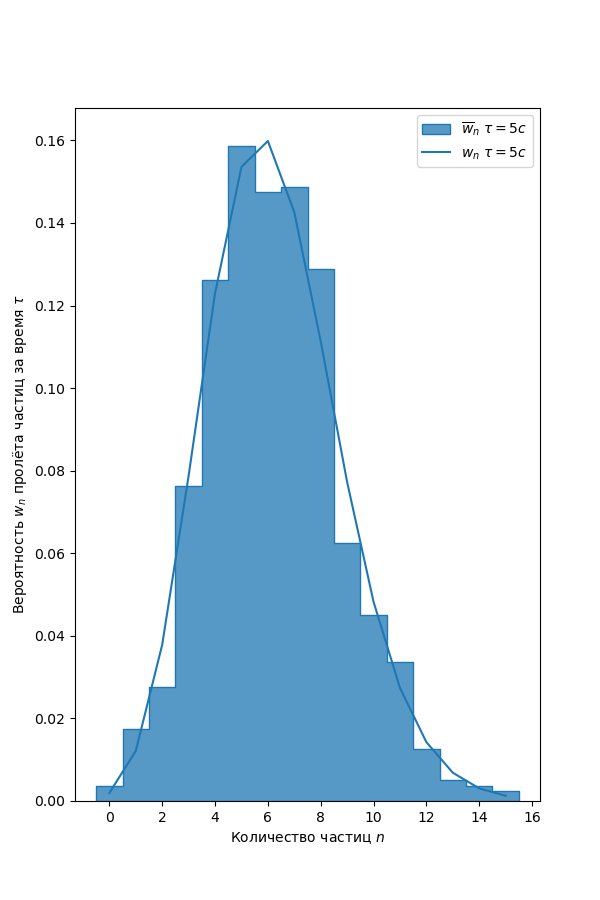
\includegraphics[width=0.45\textwidth]{imgs/5.png}} &
{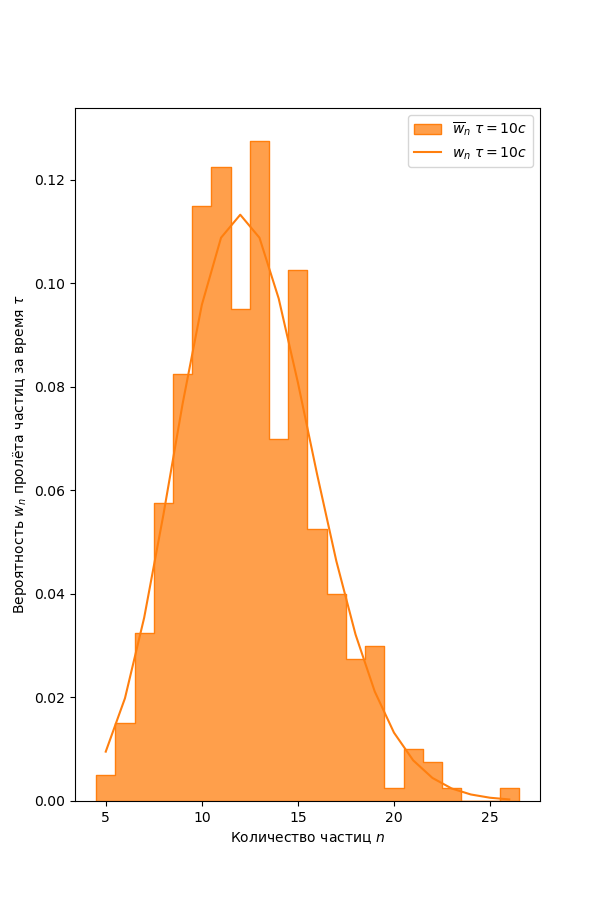
\includegraphics[width=0.45\textwidth]{imgs/10.png}} \\
{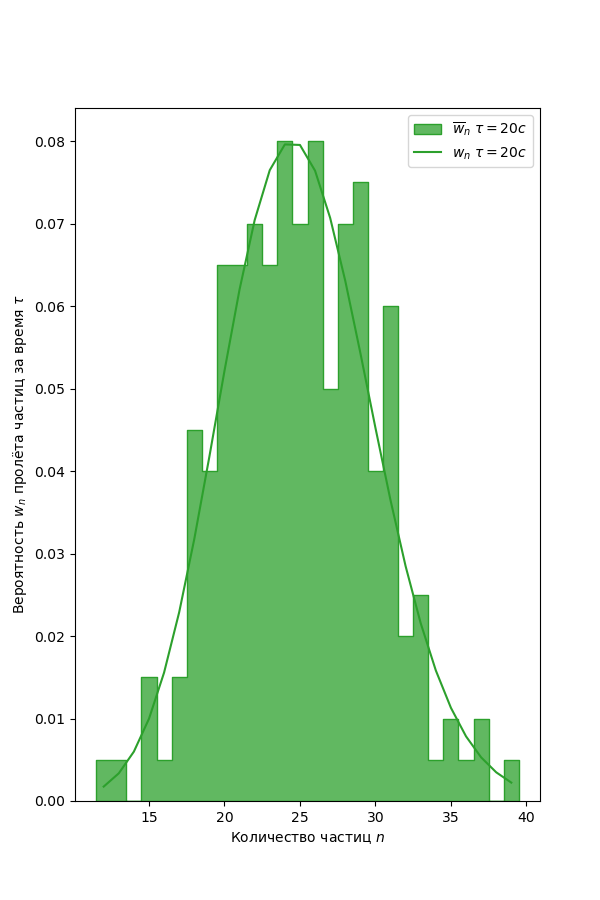
\includegraphics[width=0.45\textwidth]{imgs/20.png}} &
{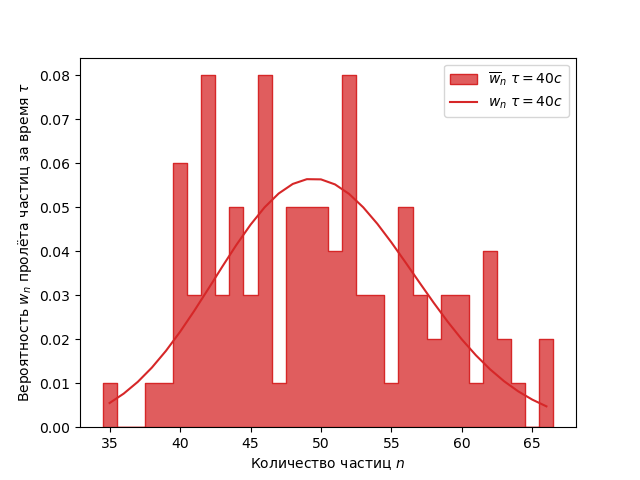
\includegraphics[width=0.45\textwidth]{imgs/40.png}} 
\end{tabular}
\caption{Гистограммы эксперимента 2 с предпологаемой кривой распределения Пуассона}
\end{figure}

\newpage

\begin{figure}[!ht]
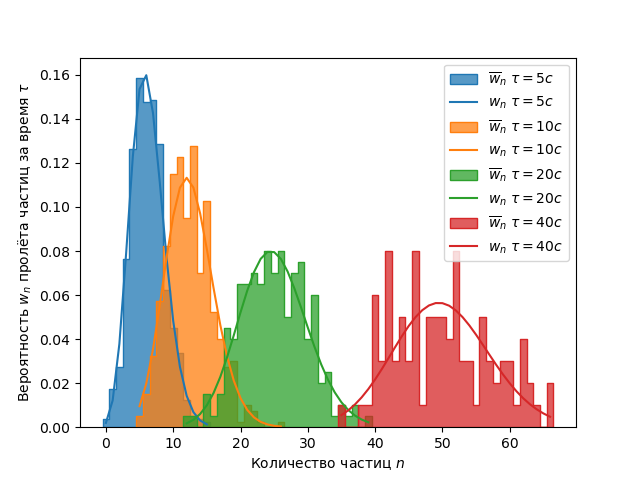
\includegraphics[width=0.825\textwidth]{imgs/all.png}
\caption{Гистограммы эксперимента 2 с предпологаемой кривой распределения Пуассона на одном графике}
\end{figure}
\begin{figure}[!ht]
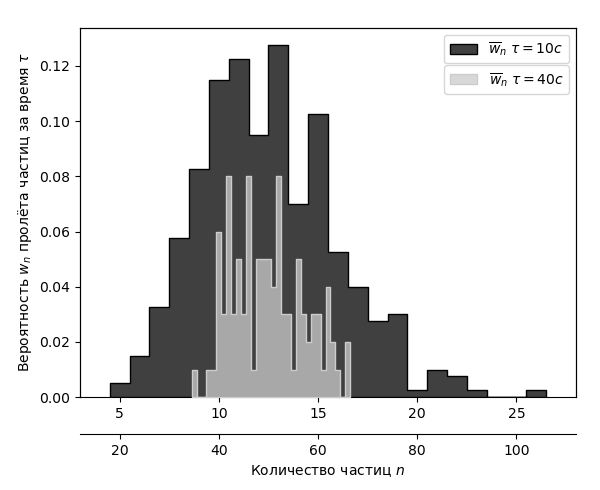
\includegraphics[width=0.825\textwidth]{imgs/hist.png}
\caption{Гистограммы эксперимента 2, наложенные друг на друга для $\tau$=10c и $\tau$=40c}
\end{figure}

\newpage

\begin{figure}[!ht]
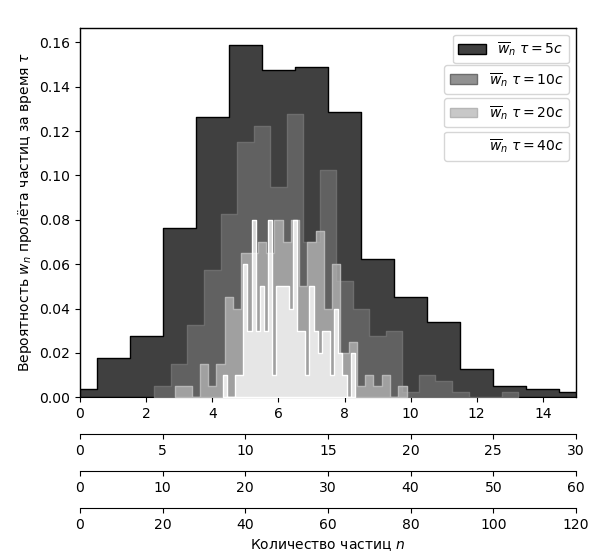
\includegraphics[width=1\textwidth]{imgs/allhist.png}
\caption{Гистограммы эксперимента 2, наложенные друг на друга}
\end{figure}

\clearpage

\subsection{Сравнение с опытом с флуктуацией плотности потока}
Проведя аналогичные расчёты гистограммы для эксперимента 1 получим, что возникает небольшая группа значений вдлаи от основного распределения (Рисю 6). А значит у нас идёт объедининие двух процессов и распределение пуассона не будет удовлетворять с достаточной точностью распределению значений. Это можно увидеть при рассмотрении графика зависимости $\varepsilon_{\sigma}$ от длины отсчёта $\tau$ (Рис 7.). При увеличении $\tau$ и при достаточных $N$ $\varepsilon_{\sigma}$ стремится к настоящему отклонению процесса от пуассоновского. И исходя из этого можно находить с помощью этого внезапные источники излучения, даже если они фиксировались непродолжительными промежутками времени.

\begin{figure}[!ht]
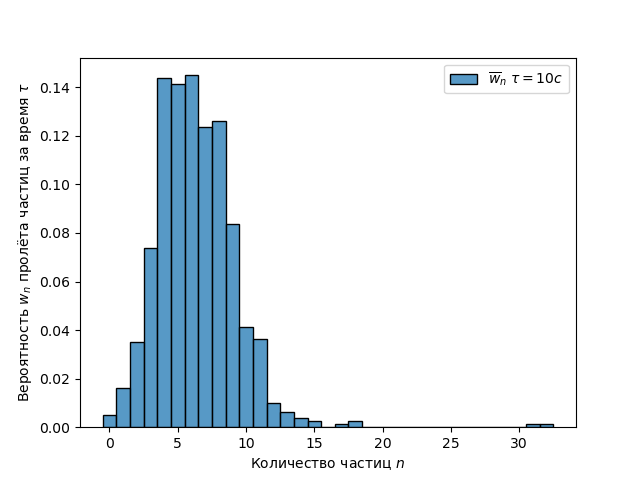
\includegraphics[width=\textwidth]{imgs/sus.png}
\caption{Гистограммы эксперимента 1 и $\tau$=10с}
\end{figure}
\begin{figure}[!ht]
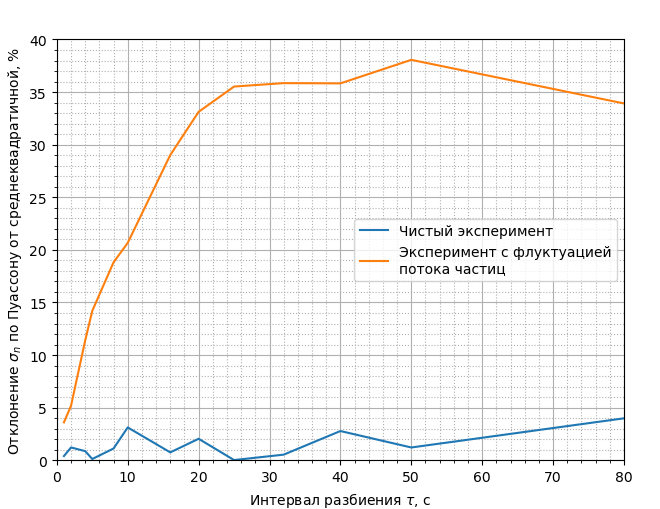
\includegraphics[width=\textwidth]{imgs/sigma.png}
\caption{График зависимости $\varepsilon_{\sigma}$ от $\tau$}
\end{figure}

\clearpage
\section{ Обсуждение результатов и выводы}
В работе получена интенсивность регестрируемых частиц в секунду и вероятности получения различных значений на датчике за $\tau$=5с, 10с, 20с, 40с. Погрешность среднего измерения >1\%, что является очень хорошим результатом. По данным мы можем сказать, что они соответствуют справочным данным о радиационном фоне и плотности космических лучей у поверхности земли. 

Эксперементально было подтверждено, что процесс фиксации космических лучей является пуассоновским, и что при достаточно большом количестве измерений можно описать его с помощью распределения Гусса. Также было обнаружено, что с помощью сравнения погрешностей измерений по оценке пуассоновского процесса и по стандартному отклонению можно определить появлялся ли инордный источник излучения.

Из проделанных измерений видно, что дальнейшее увеличение точности невозможно без увеличения времени эксперимента. Также видно, что чем больше значений для гистограммы, тем ближе она к теоретическому распределению. Примерно 200-400 отсчётов достаточно для хорошей гисстограммы.
\end{document}